\documentclass[border=5pt]{standalone}

\usepackage{tikz}
\usetikzlibrary{shapes.geometric}

\begin{document}


\begin{tikzpicture}
\node[cylinder, draw, shape aspect=.5] {ABC};
\end{tikzpicture}

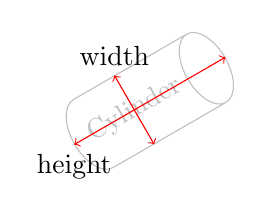
\begin{tikzpicture}
  \node [cylinder, gray!50, rotate=30, draw,
    minimum height=2cm, minimum width=1cm] (c) {Cylinder};
  \draw[red, <->] (c.top)   -- (c.bottom)
    node [at end, below, black]   {height};
  \draw[red, <->] (c.north) -- (c.south)
    node [at start, above, black] {width};
\end{tikzpicture}

\end{document}

